\section{Classification using both amplitude and phase}

Durch die Einführung der Phase ist viel mehr Information verfügbar als durch die Amplitude alleine, was die Performance der Klassifikation deutlich verbessern sollte.

\subsection{Likelihood models}

Schätzen der Normalverteilung der LOS-Phase:

$$ p(x_2 | t = \mathrm{LOS}) = \frac{1}{\sqrt{2 \pi} \sigma_{x_2}} exp(-\frac{(x - \mu_{x_2})^2}{\sigma_{x_2}^2}) $$
$$ \mu_{x_2} = \frac{1}{N_{LOS}} \sum_{x \in LOS} x $$
$$ \sigma_{x_2}^2 = \frac{1}{N_{LOS}} \sum_{x \in LOS} (x - \mu_{x_2})^2 $$

Die Verteilung der NLOS-Phase ist uniform:

$$ p(x_2 | t = \mathrm{NLOS}) = \frac{1}{2 \pi} $$

Abbildung \ref{fig:5_1_2_estimation} zeigt die ermittelten Schätzwerte für die Verteilungen der Phase. Man erkennt, dass die Schätzwerte gut mit den Testdaten übereinstimmen.

\begin{figure}[h!]
  \centering
  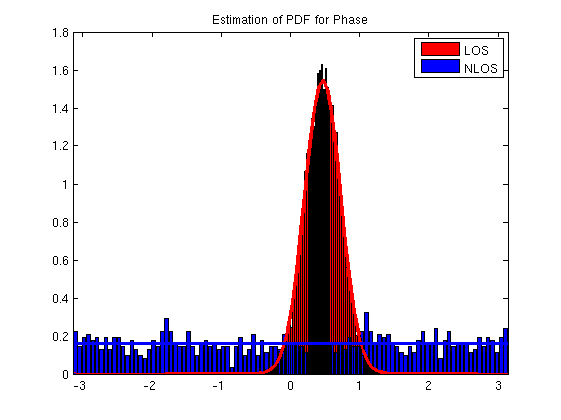
\includegraphics[width=0.75\textwidth]{./figures/5_1_2_estimation.png}
  \caption{Normalisierte Histogramme der geschätzen Verteilungen der Phase}
  \label{fig:5_1_2_estimation}
\end{figure}


\subsection{ML-Klassifikation}

Abbildung \ref{fig:5_1_2_ml} zeigt die Klassifikation mit ML. Durch die zusätzliche Information der Phase können die beiden Bereiche besser unterschieden werden als nur durch die Amplitude. Die Erkennung funktioniert in diesem Beispiel schon recht gut, ein gewisser Bereich (linker Bereich von LOS) wird jedoch noch falsch klassifiziert.

\texttt{ML: Es wurden 95.0091\% korrekt klassifiziert}

\begin{figure}[h!]
  \centering
  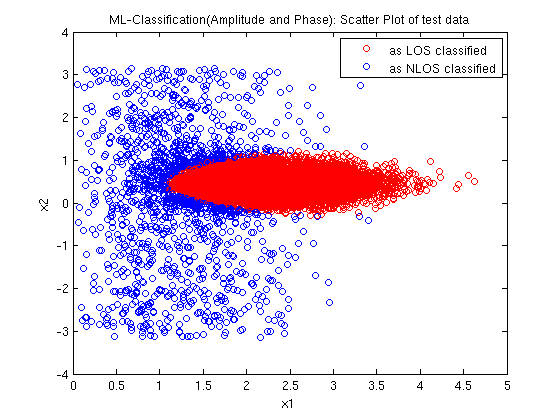
\includegraphics[width=0.75\textwidth]{./figures/5_1_2_ml.png}
  \caption{Klassifikation der Daten durch Most Likelihood Schätzer}
  \label{fig:5_1_2_ml}
\end{figure}


\subsection{Bayes-Klassifikation}

Abbildung \ref{fig:5_1_2_bayes} zeigt die Klassifikation mit Bayes. Wie beim ML-Schätzer ist die Klassifikation besser als ohne Phaseninformation. Die Erkennung funktioniert mit Bayes-Klassifikator noch etwas besser als mit ML, da hier auch der vorher falsch klassifizierte Bereich richtig erkannt wird.

\texttt{Bayes: Es wurden 97.5636\% korrekt klassifiziert}

\begin{figure}[h!]
  \centering
  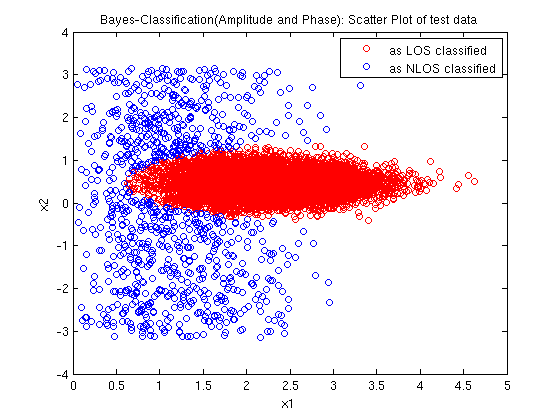
\includegraphics[width=0.75\textwidth]{./figures/5_1_2_bayes.png}
  \caption{Klassifikation der Daten durch Bayes Schätzer}
  \label{fig:5_1_2_bayes}
\end{figure}
